\documentclass[%
 reprint,
 amsmath,
 amssymb,
 showkeys,
 pra,
 floatfix,
 onecolumn,
]{revtex4-2}

\usepackage{xr}

\renewcommand\thefigure{S\arabic{figure}}
\renewcommand\thesection{S\arabic{section}}

\usepackage[linesnumbered,ruled,vlined]{algorithm2e}
\let\oldnl\nl
\newcommand{\nonl}{\renewcommand{\nl}{\let\nl\oldnl}}
\usepackage{braket}
\usepackage{float}
\usepackage{xcolor}
\usepackage{color}
\usepackage{graphicx}
\usepackage{dcolumn}
\usepackage{enumitem}
\usepackage{lipsum}  
\usepackage{bm}
\usepackage{hyperref}
\hypersetup{
    colorlinks=true,
    linkcolor=blue,
    citecolor=magenta
}
\usepackage{subcaption}
\usepackage{listings}
\captionsetup{justification = raggedright, singlelinecheck = true}

% Default fixed font does not support bold face
\DeclareFixedFont{\ttb}{T1}{txtt}{bx}{n}{10} % for bold
\DeclareFixedFont{\ttm}{T1}{txtt}{m}{n}{10}  % for normal
\definecolor{deepblue}{rgb}{0,0,0.5}
\definecolor{deepred}{rgb}{0.6,0,0}
\definecolor{deepgreen}{rgb}{0,0.5,0}
\definecolor{light-gray}{gray}{0.95}
\lstset{
    language=Python,
    basicstyle=\ttm,
    morekeywords={self},              % Add keywords here
    keywordstyle=\ttb\color{deepblue},
    emph={MyClass,__init__},          % Custom highlighting
    emphstyle=\ttb\color{deepred},    % Custom highlighting style
    stringstyle=\color{deepgreen},
    showstringspaces=false,
    xleftmargin=.55cm,
    backgroundcolor =\color{light-gray},
}
        

\begin{document}

\preprint{APS/123-QED}
\title{Supplementary: qLEET - Visualizing Loss Landscapes, Expressibility, Entangling power and Training Trajectories for Parameterized Quantum Circuits}

\author{Utkarsh Azad}
\email{utkarsh.azad@research.iiit.ac.in}
\thanks{Corresponding Author}
\author{Animesh Sinha}
\email{animesh.sinha@research.iiit.ac.in}
\affiliation{
    Center for Computational Natural Sciences and Bioinformatics, International Institute of Information Technology, Hyderabad.\\
    Center for Quantum Science and Technology,\\ International Institute of Information Technology, Hyderabad.
}
\date{\today}

\maketitle

\section{\label{sec:supl-expressibility-tutorial}Tutorial: Entaglement Ability Analysis}

In this section, we will learn how to calcualte expressibility of Parameterized Quantum Circuits (PQCs) using qLEET, which could thought of as traversing power of a PQC in the Hilbert space. We look at different parameterized states generated by the sampled ensemble of parameters for a given PQC. We then compare the resulting distribution of state fidelities ($\mathcal{F}$) generated by this sampled ensemble to that of the ensemble of Haar random states.

We currently support two expressibility measures - \textbf{Kullback–Leibler Divergence} and \textbf{Jensen–Shannon Divergence}
$$ \textrm{Expressibility} = D_{\textrm{KL}} \Big( \hat{P}_{\textrm{PQC}}(\mathcal{F}; \theta) \big\vert P_{\textrm{Haar}}(\mathcal{F}) \Big) $$
$$ \textrm{Expressibility} = D_{\sqrt{\textrm{JSD}}} \Big( \hat{P}_{\textrm{PQC}}(\mathcal{F}; \theta) \big\vert P_{\textrm{Haar}}(\mathcal{F}) \Big) $$

All circuit analysis using qleet begins with defining a parameterized quantum circuit using a library of choice, and then passing it into qleet's \lstinline{CircuitDescriptor} interface.

\begin{lstlisting}
params = [qiskit.circuit.Parameter(r"$\theta_1$")]

qiskit_circuit = qiskit.QuantumCircuit(1)
qiskit_circuit.h(0)
qiskit_circuit.rz(params[0], 0)
qiskit_descriptor = qleet.interface.circuit.CircuitDescriptor(
    circuit=qiskit_circuit, params=params, cost_function=None
)
\end{lstlisting}

The analyze the expressibility, we can use the corresponding analyzer. We can get the expressibility using either of the two supported measures.

\begin{lstlisting}

qiskit_expressibility = qleet.analyzers.expressibility.Expressibility(
    qiskit_descriptor, samples=100
)
expr_jsd = qiskit_expressibility.expressibility("jsd")
print("JSD Expressibility:", expr_jsd)

expr_kld = qiskit_expressibility.expressibility("kld")
print("KLD Expressibility:", expr_kld)

plt_figure = qiskit_expressibility.plot()
\end{lstlisting}

We look at different parameterized states generated by the sampled ensemble of parameters for a given PQC. We then compare the resulting distribution of eigenvalues of the bipartite state generated by this sampled ensemble to that of the ensemble of eigenvalues of Haar random states.

We currently support two measures to calculate entanglement spectrum divergence (ESD) - \textbf{Kullback–Leibler Divergence} and \textbf{Jensen–Shannon Divergence}
$$\textrm{ESD} = D_{\textrm{KL}} \Big(\hat{P}_{\textrm{PQC}}(H_{\textrm{ent}}; \theta) \big\vert P_{\textrm{Haar}}(H_{\textrm{ent}}) \Big) $$
$$\textrm{ESD} = D_{\sqrt{\textrm{JSD}}} \Big(\hat{P}_{\textrm{PQC}}(H_{\textrm{ent}}; \theta) \big\vert P_{\textrm{Haar}}(H_{\textrm{ent}}) \Big) $$

\begin{lstlisting}
params = [
    qiskit.circuit.Parameter(r"$\theta_1$"),
    qiskit.circuit.Parameter(r"$\theta_2$")
]
qiskit_circuit = qiskit.QuantumCircuit(2)
qiskit_circuit.rx(params[0], 0)
qiskit_circuit.cx(0, 1)
qiskit_circuit.rx(params[1], 1)
qiskit_descriptor = qleet.interface.circuit.CircuitDescriptor(
    circuit=qiskit_circuit, params=params, cost_function=None
)
\end{lstlisting}

\begin{lstlisting}
analyzer = (
    qleet.analyzers.entanglement.EntanglementCapability(
        qiskit_descriptor, samples=500
    )
)

entanglement_mw = analyzer.entanglement_capability("meyer-wallach")
print("Entanglement Capability (Meyer Wallach Measure):", entanglement_mw)

entanglement_scott = analyzer.entanglement_capability("scott")
print("Entanglement Capability (Scott Measure):", entanglement_scott)
\end{lstlisting}

In this section, we will plot the entanglement spectrum.

\begin{lstlisting}
def ansatz(params, cparams=None):
    layers, num_qubits, depth = params.shape
    ansatz = qiskit.QuantumCircuit(num_qubits)
    for idx in range(layers):
        if idx:
            ansatz.barrier()
        for ind in range(num_qubits):
            ansatz.rx(params[idx][ind][0], ind)
            ansatz.rz(params[idx][ind][1], ind)
            ansatz.rx(params[idx][ind][2], ind)
        for ind in range(num_qubits-1):
            ansatz.cx(ind, ind+1)
    return ansatz
\end{lstlisting}

\begin{lstlisting}
data = []
results = []
num_qubits = 12
for idx in range(1, 17):
    print(idx, end=' ')
    params = np.array([qiskit.circuit.Parameter(fr"$\theta_{idx}$")
                       for idx in range(idx*num_qubits*3)])
    qiskit_descriptor = qleet.CircuitDescriptor(
        circuit=ansatz(np.array(params).reshape((idx, num_qubits, 3))), 
        params=params, cost_function=None
    )
    qiskit_entanglement_spectrum = \
        qleet.analyzers.entanglement_spectrum.EntanglementSpectrum(
            qiskit_descriptor, samples=100
        )
    pqc_esd, mean_eig = qiskit_entanglement_spectrum.entanglement_spectrum("jsd")
    results.append(pqc_esd)
    data.append(mean_eig)
data = np.array(data)

fig = qiskit_entanglement_spectrum.plot(data)
\end{lstlisting}

\section{\label{sec:supl-loss-tutorial}Loss Landscape and Training Trajectory Analysis}

For this section of the tutorial, we shall be constructing our circuits in the \textbf{Cirq} library, which is also supported by our multi-backend analyzer. Using cirq, we define a parameterized quantum circuit, we define its parameters as sympy symbols, and we define a cost function as a Pauli measurement on the outputs of this circuits. All of this is passed into out \lstinline{CircuitDescriptor} interface

\begin{lstlisting}
graph = nx.gnm_random_graph(n=8, m=20)
qubits = cirq.GridQubit.rect(1, graph.number_of_nodes())
p = 5

params = sympy.symbols("q0:%d" % (2 * p))
qaoa_circuit = cirq.Circuit()
for qubit in qubits:
    qaoa_circuit.append(cirq.H(qubit))
for i in range(p):
    for edge in graph.edges():
        qaoa_circuit += cirq.CNOT(qubits[edge[0]], qubits[edge[1]])
        qaoa_circuit += cirq.rz(params[2 * i]).on(qubits[edge[1]])
        qaoa_circuit += cirq.CNOT(qubits[edge[0]], qubits[edge[1]])
    for j in range(len(qubits)):
        qaoa_circuit += cirq.rx(2 * params[2 * i + 1]).on(qubits[j])

qaoa_cost = cirq.PauliSum()
for edge in graph.edges():
    qaoa_cost += cirq.PauliString(1 / 2 * cirq.Z(qubits[edge[0]]) * 
                                  cirq.Z(qubits[edge[1]]))

circuit = qleet.interface.circuit.CircuitDescriptor(
    qaoa_circuit, params, qaoa_cost)
solver = qleet.simulators.pqc_trainer.PQCSimulatedTrainer(circuit)
\end{lstlisting}

\begin{lstlisting}
class MaxCutMetric(qleet.interface.metric_spec.MetricSpecifier):

    def __init__(self, graph):
        super().__init__("samples")
        self.graph = graph

    def from_samples_vector(self, samples_vector):
        return np.mean([nx.algorithms.cuts.cut_size(
            self.graph, np.where(cut)[0]) for cut in samples_vector])
    
    def from_density_matrix(self, density_matrix):
        raise NotImplementedError
    
    def from_state_vector(self, state_vector):
        raise NotImplementedError

metric = MaxCutMetric(graph)
\end{lstlisting}

\begin{lstlisting}
plot = qleet.analyzers.loss_landscape.LossLandscapePlotter(
    solver, metric, dim=2)
solver.train(n_samples=5000)
fig_loss_surface = plot.plot("surface", points=20)

trackers = qleet.interface.metas.AnalyzerList(
    qleet.analyzers.training_path.LossLandscapePathPlotter(plot),
    qleet.analyzers.training_path.OptimizationPathPlotter(mode="tSNE"),
)
for _i in range(5):
    solver.train(loggers=trackers, n_samples=5000)
    trackers.next()
    
fig_loss_traversal = trackers[0].plot()
fig_training_trace = trackers[1].plot()
\end{lstlisting}

\begin{figure*}[htp]
    \centering
    \begin{subfigure}[b]{0.32\linewidth}
        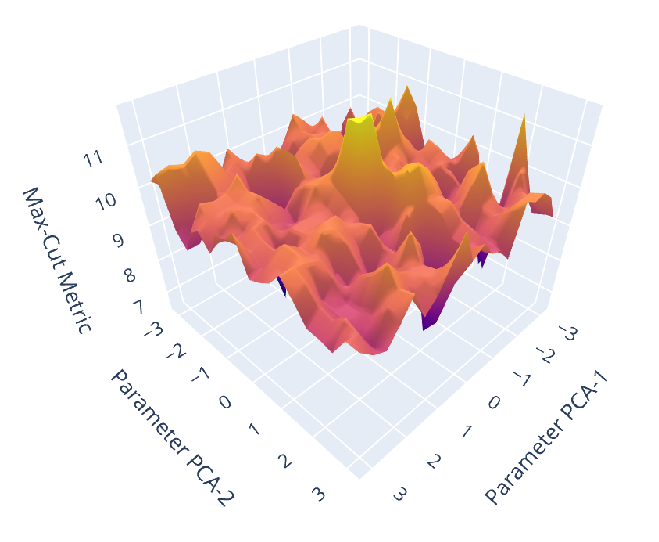
\includegraphics[width=\textwidth]{images/supplementary-qleet-1.pdf}
        \caption{Metric Landscape (inverse of loss) around obtained optima}
    \end{subfigure}
    \begin{subfigure}[b]{0.32\linewidth}
        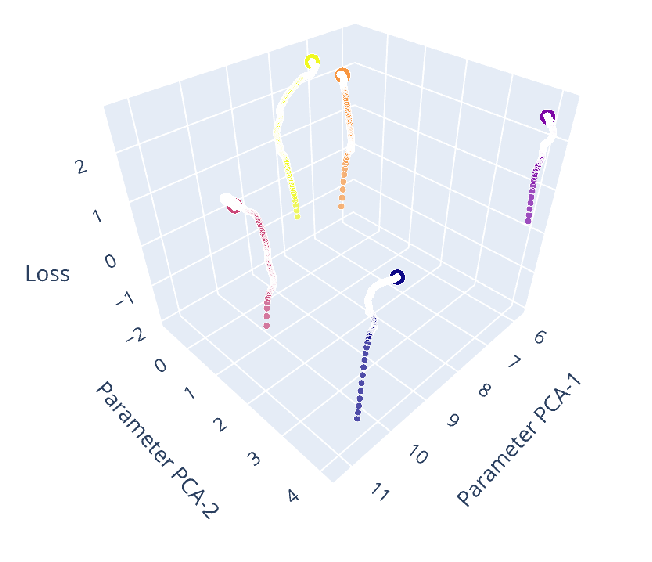
\includegraphics[width=\textwidth]{images/supplementary-qleet-2.pdf}
        \caption{PCA plot with loss for training trajectories of 5 runs}
    \end{subfigure}
    \begin{subfigure}[b]{0.32\linewidth}
        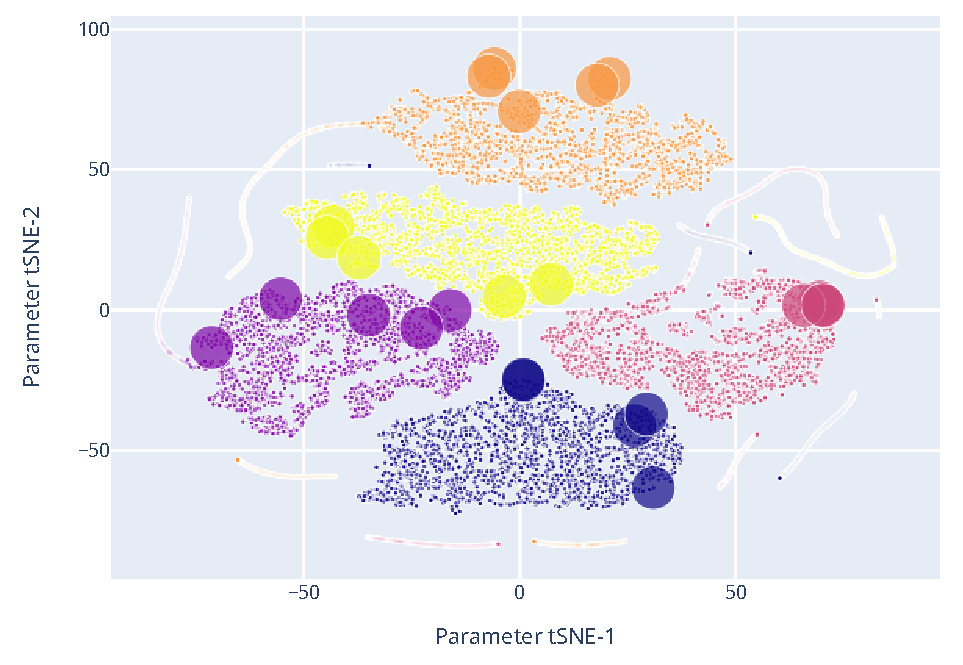
\includegraphics[width=\textwidth]{images/supplementary-qleet-3.pdf}
        \caption{2-D tSNE of training trajectories from 5 runs}
    \end{subfigure}%
    \caption{Loss and Training Trajectory plots obtained on analyzing the circuit shown. Here, the analysis is shown for a circuit representing max-cut on a graph with 8 nodes and 20 edges.}
    \label{fig:loss-land-train-traj}
\end{figure*}

\section{\label{sec:supl-mz-op}Entanglement Analysis for $M_Z$ operator \cite{Zidan2020}}

\begin{figure}
    \centering
    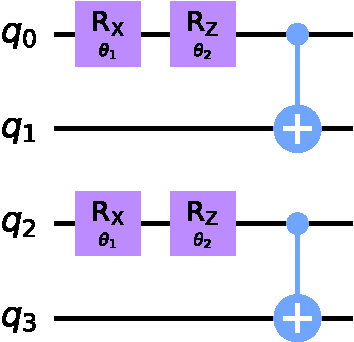
\includegraphics{images/mzop_circuit.pdf}
    \caption{$M_Z$ operator used in the quantum computing model based on entanglement degree allows to differentiate between the non-orthogonal states of the form $e_1|0\rangle + e_2|1\rangle$, with arbitrary accuracy \cite{Zidan2020, Khan2022, Punla2021, Panda2022}.}
    \label{fig:my_label}
\end{figure}

\begin{lstlisting}
params = [qiskit.circuit.Parameter(r"$\theta_1$"), 
          qiskit.circuit.Parameter(r"$\theta_2$"), 
          qiskit.circuit.Parameter(r"$\theta_3$"), 
          qiskit.circuit.Parameter(r"$\theta_4$")]

qiskit_circuit = qiskit.QuantumCircuit(4)
qiskit_circuit.rx(params[0], 0)
qiskit_circuit.rz(params[1], 0)
qiskit_circuit.rx(params[2], 2)
qiskit_circuit.rz(params[3], 2)
qiskit_circuit.cx(0, 1)
qiskit_circuit.cx(2, 3)

qiskit_descriptor = qleet.interface.circuit.CircuitDescriptor(
    circuit=qiskit_circuit, params=params, cost_function=None
)

qiskit_entg_capability = (
    qleet.analyzers.entanglement.EntanglementCapability(
        qiskit_descriptor, samples=1000
    )
)

entanglement_mw = qiskit_entg_capability.entanglement_capability("meyer-Wallach")
# >>> entanglement_mw = 0.5010648894421558

entanglement_scott = qiskit_entg_capability.entanglement_capability("scott")
# >>> entanglement_scott = array([0.4979689 , 0.38654991])


\end{lstlisting}

\section{Quantum Circuits from the Experiments}

\subsection{Loss Landscape and Training Trajectories (Fig. \ref{fig:qaoa-circuit} $\rightarrow$ Fig. 3)}
\begin{figure}[!ht]
    \centering
    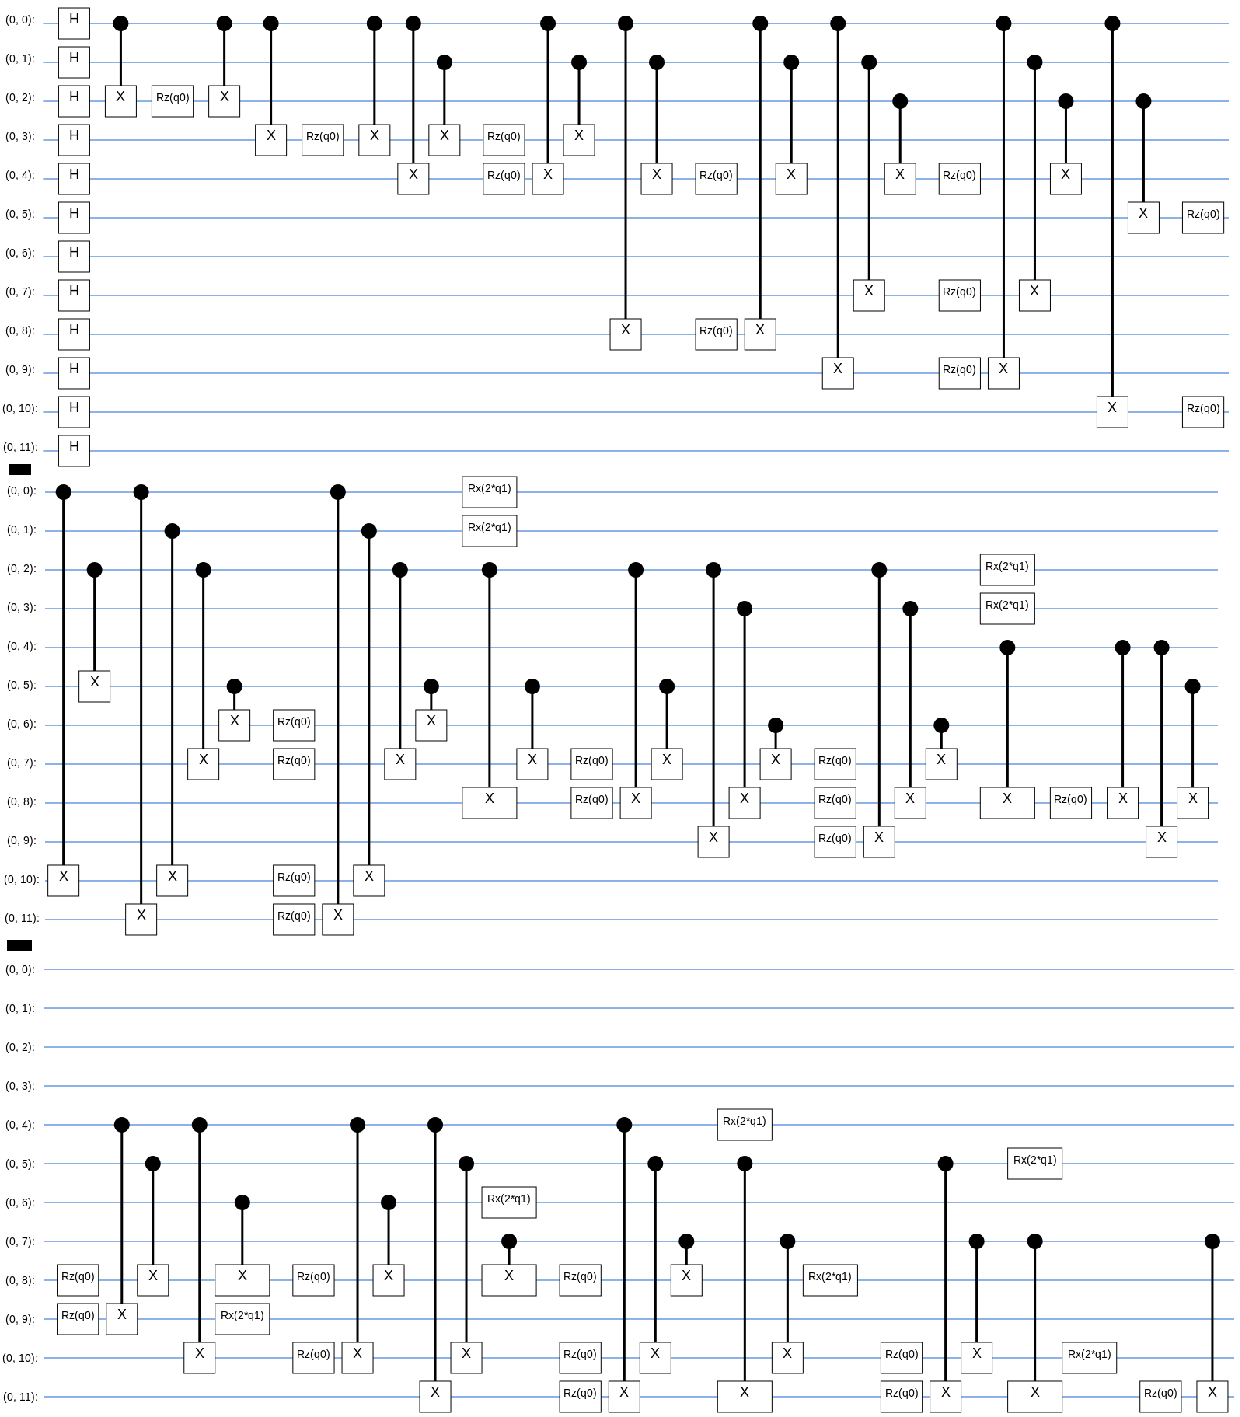
\includegraphics[width=\textwidth]{images/qaoa-circuit.pdf}
    \caption{QAOA circuit for p=1. This circuit (except the first Hadamard layer) will be repeated $k$ times for $p=k$.}
    \label{fig:qaoa-circuit}
\end{figure}

\subsection{Expressibility (Fig. \ref{fig:expr-circuit} $\rightarrow$ Fig. 5)}
\begin{figure}[!ht]
    \centering
    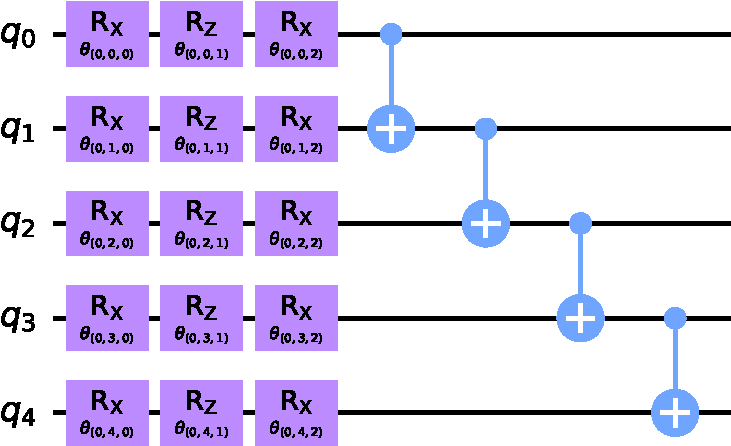
\includegraphics[width=0.5\textwidth]{images/expr_circuit.pdf}
    \caption{Parameterized quantum circuit $U(\vec{\theta}) =  \prod_{1}^{L}\big(\bigotimes_{i=1}^{5}R_x(\theta_i^1)R_z(\theta_i^2)R_x(\theta_i^3) \ldots \bigotimes_{i<j}CX(i, j)\big)$}
    \label{fig:expr-circuit}
\end{figure}


\subsection{Entangling Capability (Fig. \ref{fig:entg-circuit} $\rightarrow$ Fig. 6)}
\begin{figure}[!h]
    \centering
    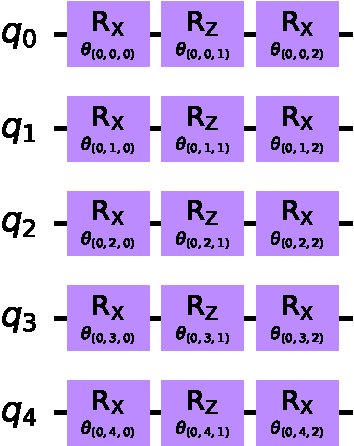
\includegraphics[width=0.25\textwidth]{images/entg_circuit.pdf}
    \caption{Parameterized quantum circuit $U(\vec{\theta}) = \bigotimes_{i=1}^{5}R_x(\theta_i^1)R_z(\theta_i^2)R_x(\theta_i^3)$}
    \label{fig:entg-circuit}
\end{figure}

\subsection{Entanglement Spectrum (Fig. \ref{fig:spec-circuit} $\rightarrow$ Fig. 7)}
\begin{figure}[!h]
    \centering
    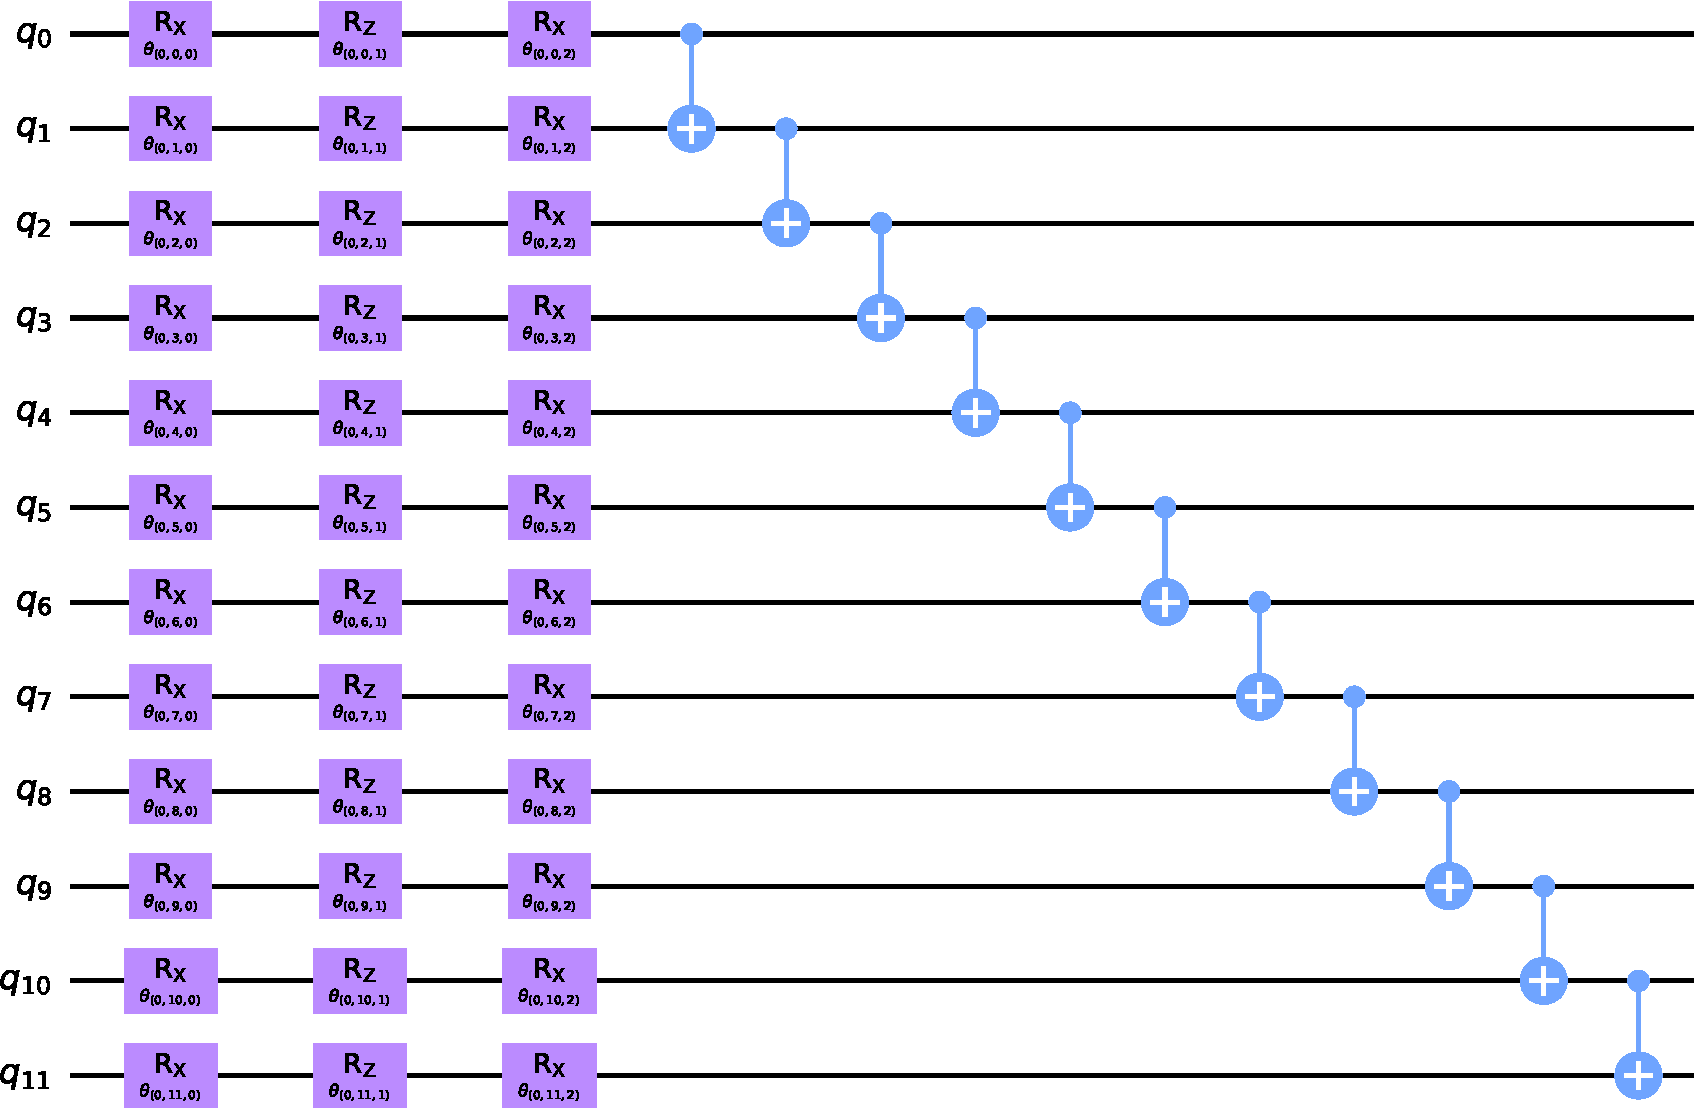
\includegraphics[width=\textwidth]{images/spec_circuit.pdf}
    \caption{Parameterized quantum circuit $U(\vec{\theta}) = \prod_{1}^{L}\big(\bigotimes_{i=1}^{12}R_x(\theta_i^1)R_z(\theta_i^2)R_x(\theta_i^3) \ldots \bigotimes_{i=1}^{11}CX(i, i+1)\big)$}
    \label{fig:spec-circuit}
\end{figure}


\bibliographystyle{apsrev4-2}
%\bibliographystyle{unsrt}


\bibliography{qleet}% Produces the bibliography via BibTeX.

\end{document}

